%!TEX root = ../Thesis.tex
\chapter{GitHub Repository}\label{cha:appendix-github}
In the following GitHub repository, you can find all relevant documentation, files and material for the project. It also contains the result analysis with the questionnaire answers in the form of a CSV file, which then was analyzed using a Jupyter Notebook. The Notebook can be found in the repository as well. Additionally can all of the raw numerical data from the objective analysis be found here. The repository also contains a wiki with more casual notes that have been made throughout the project period leading up to this final report, along with more lively media showing off the experimental application (video/GIFs). 

\begin{displayquote}
    \large \textbf{https://github.com/petrepa/TFE4940}
\end{displayquote}

%\chapter{Pre-Testing Questionnaire}\label{cha:appendix-pre-testing}
%\includepdf[pages=-]{Questionnaires/pre_testing_questionnaire.pdf}

%\chapter{Post-Testing Questionnaire}\label{cha:appendix-post-testing}
%\includepdf[pages=-]{Questionnaires/post_testing_questionnaire.pdf}

\chapter{Backgrounds used in video}\label{cha:appendix-backgrounds}
\begin{figure}[H]
    \centering
    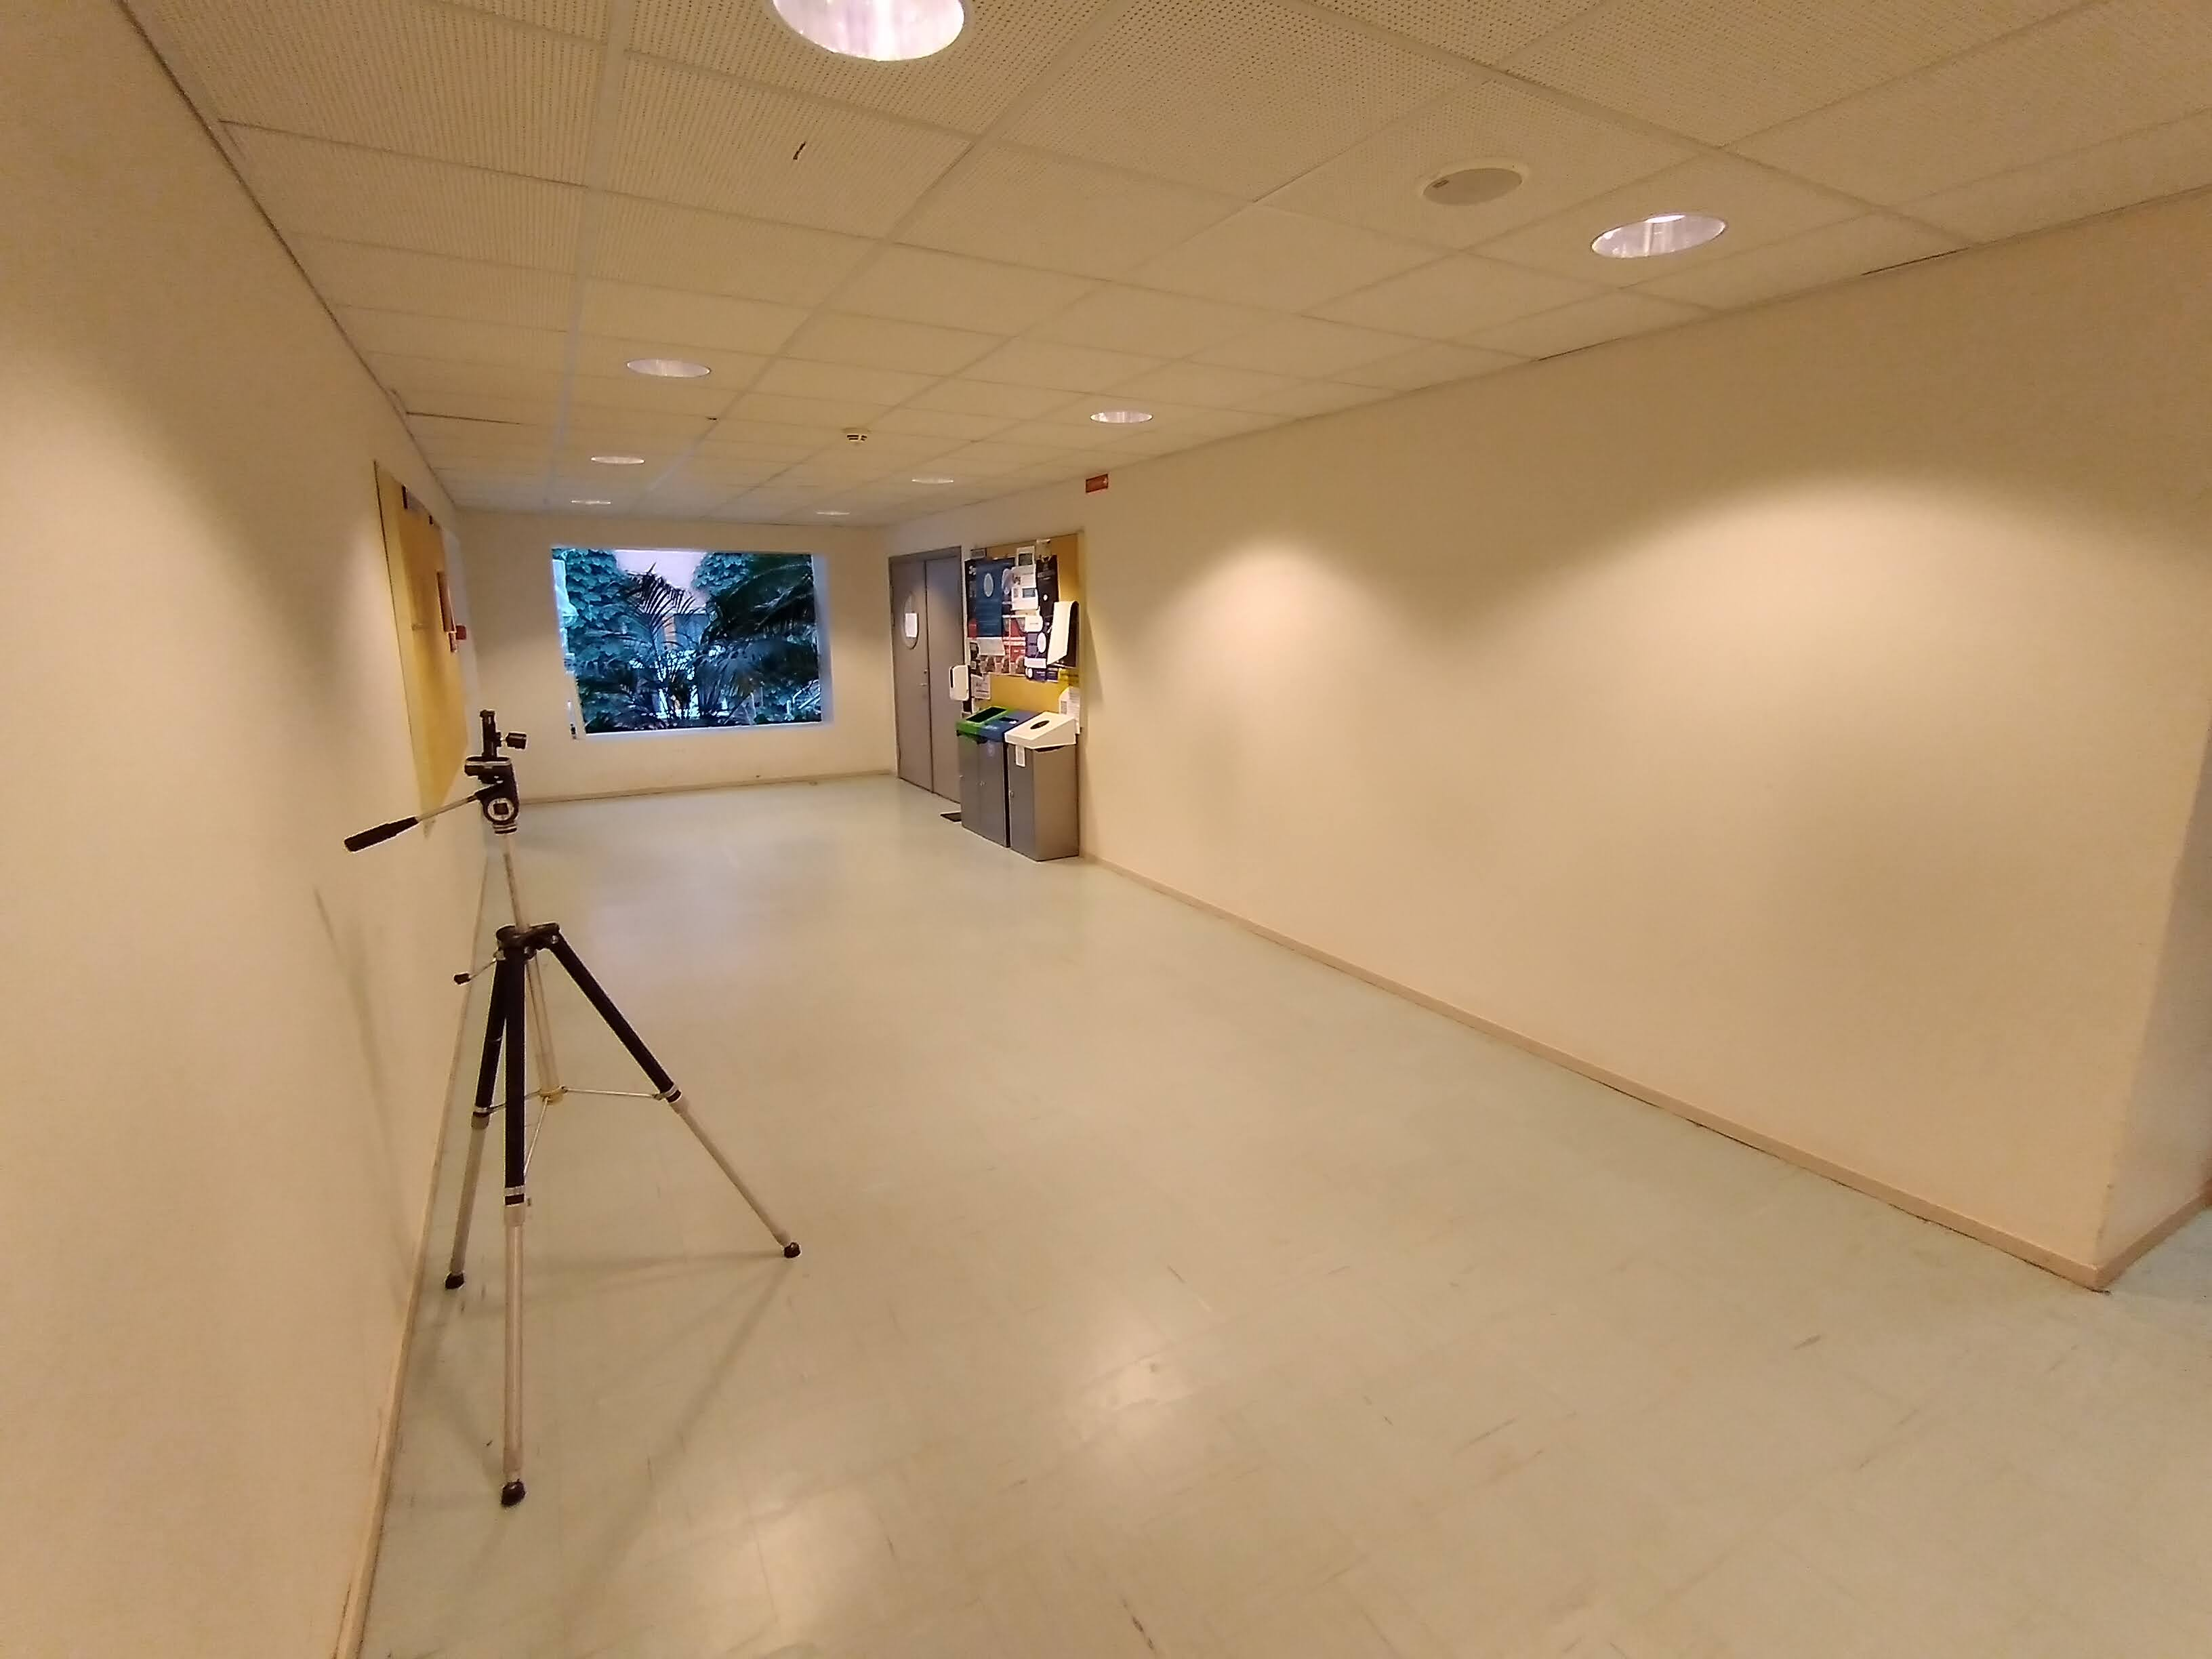
\includegraphics[width=\textwidth]{img/background_setup/simple_white_wall.jpg}
    \caption{Simple white wall}
    \label{fig:white_wall_setup}
\end{figure}
\begin{figure}[H]
    \centering
    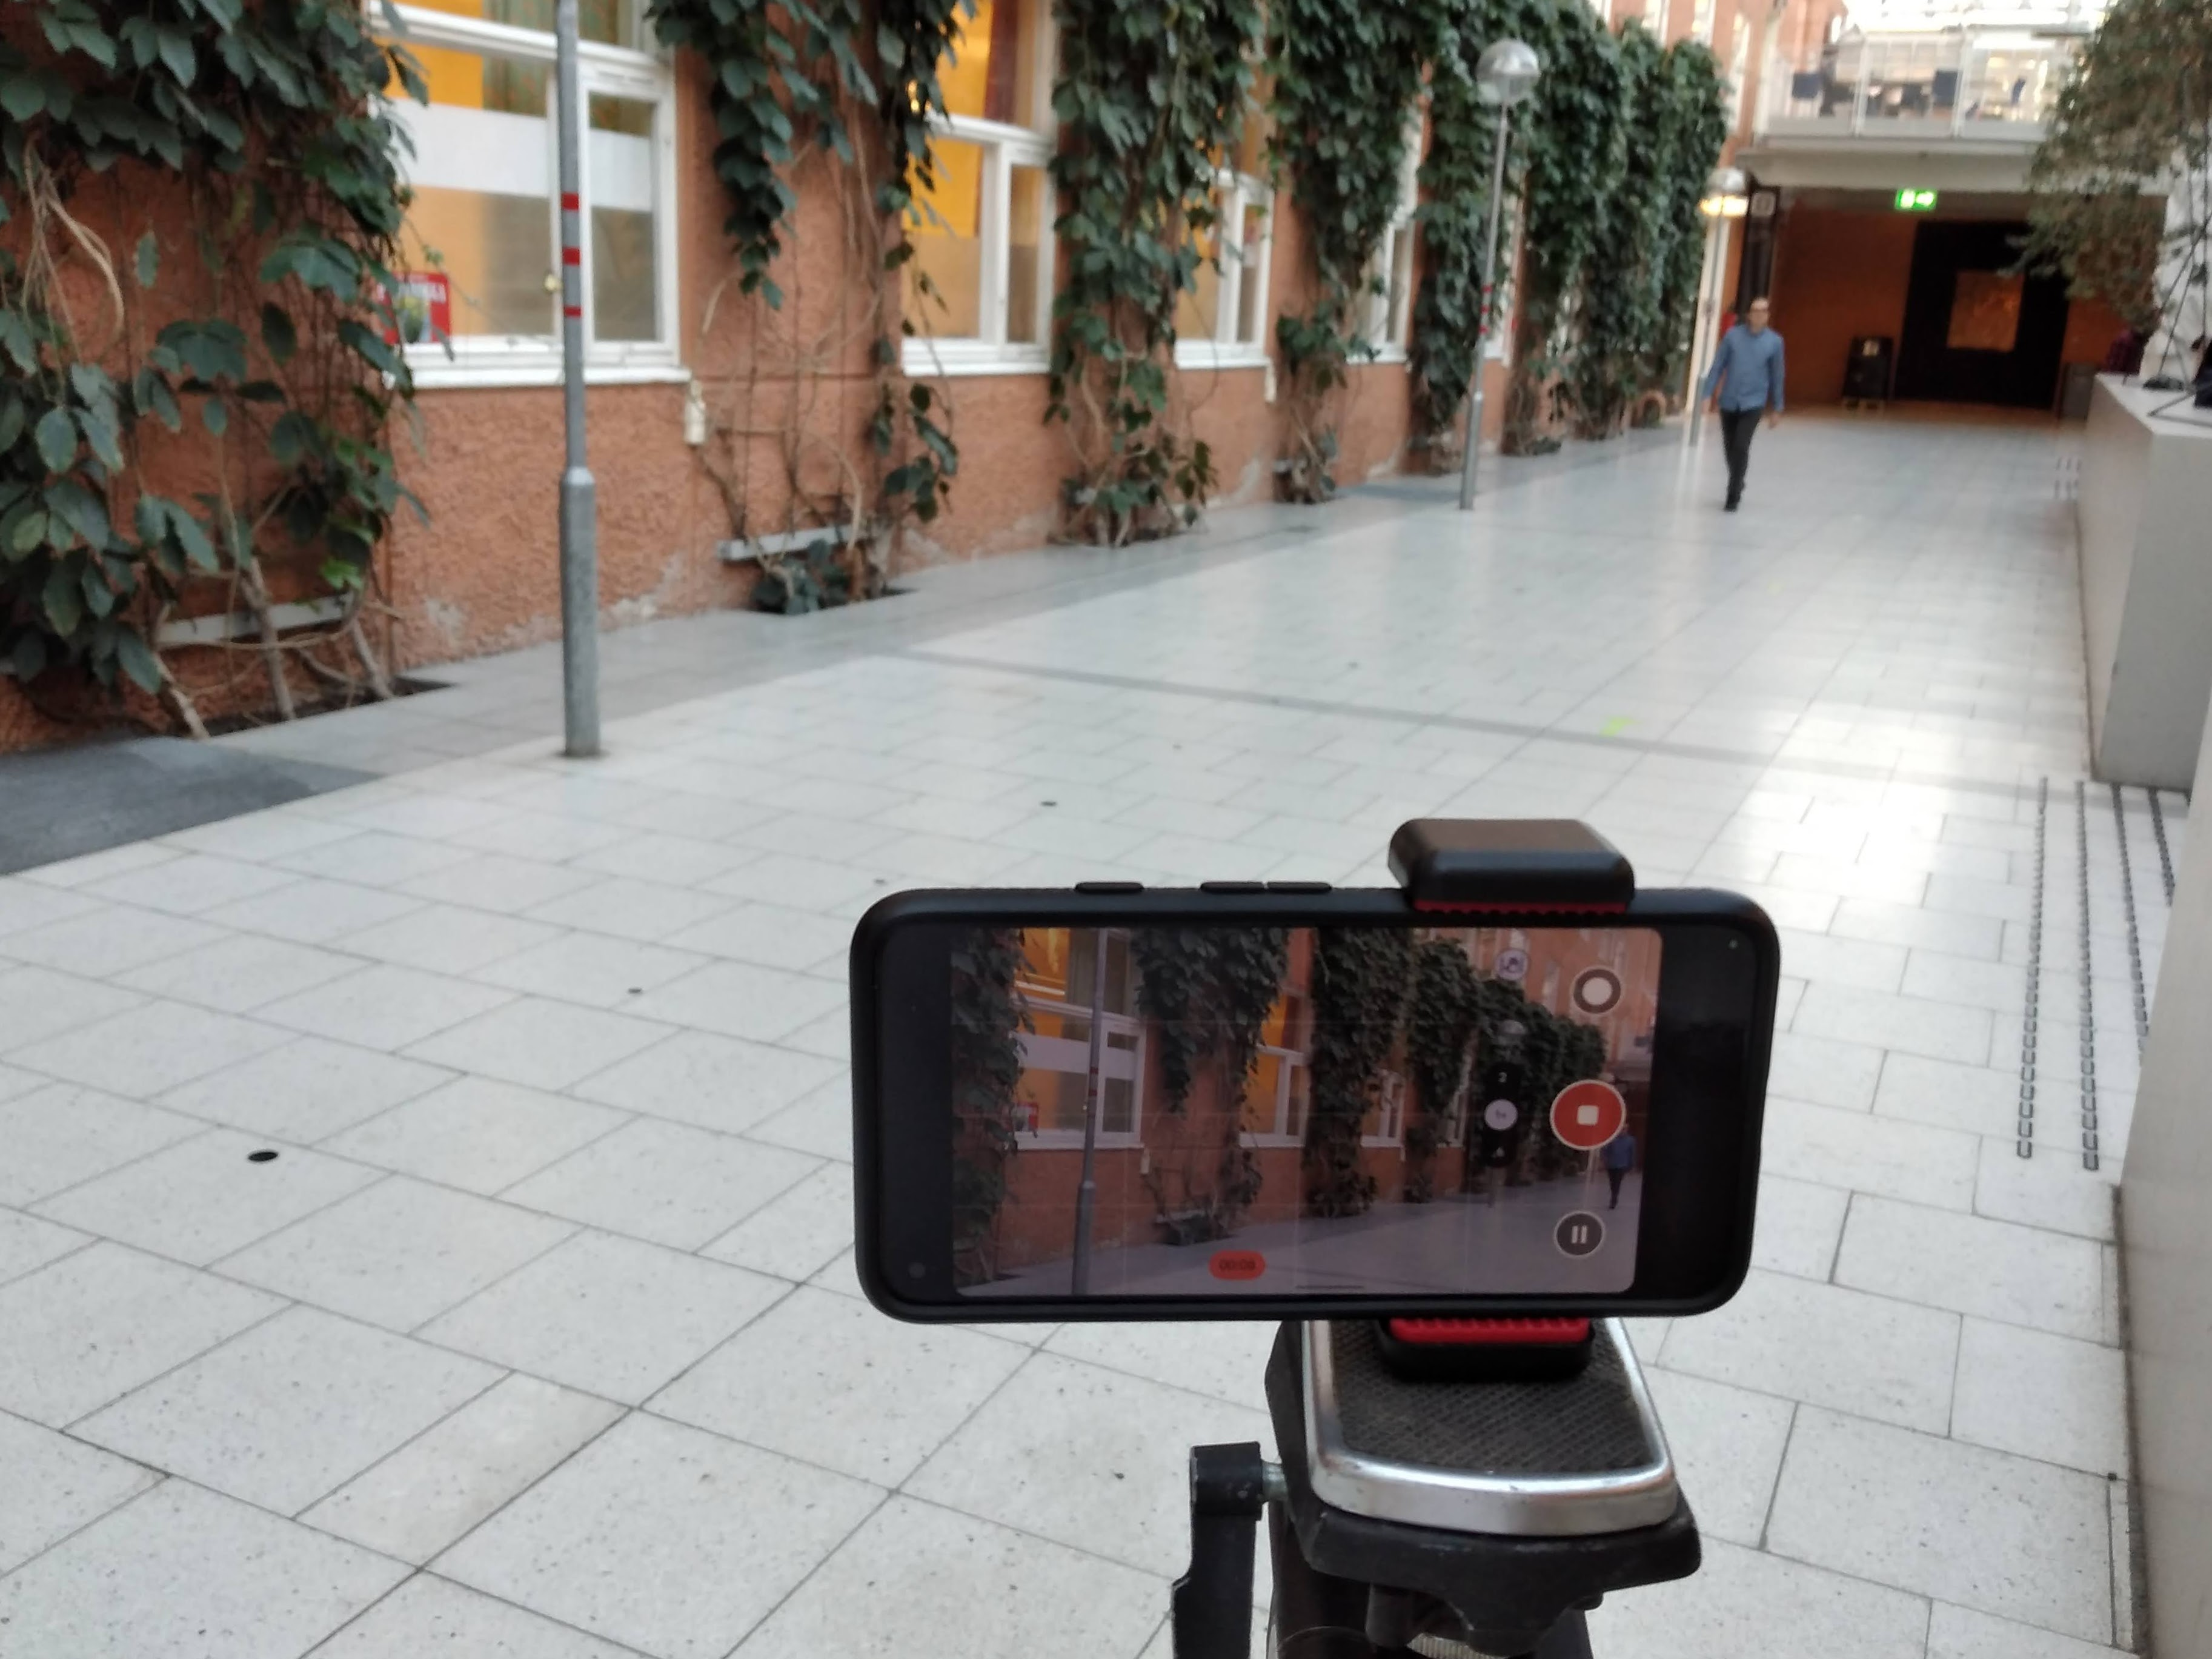
\includegraphics[width=\textwidth]{img/background_setup/complex_wall.jpg}
    \caption{Complex wall with different colors and textures}
    \label{fig:complex_setup}
\end{figure}
\begin{figure}[H]
    \centering
    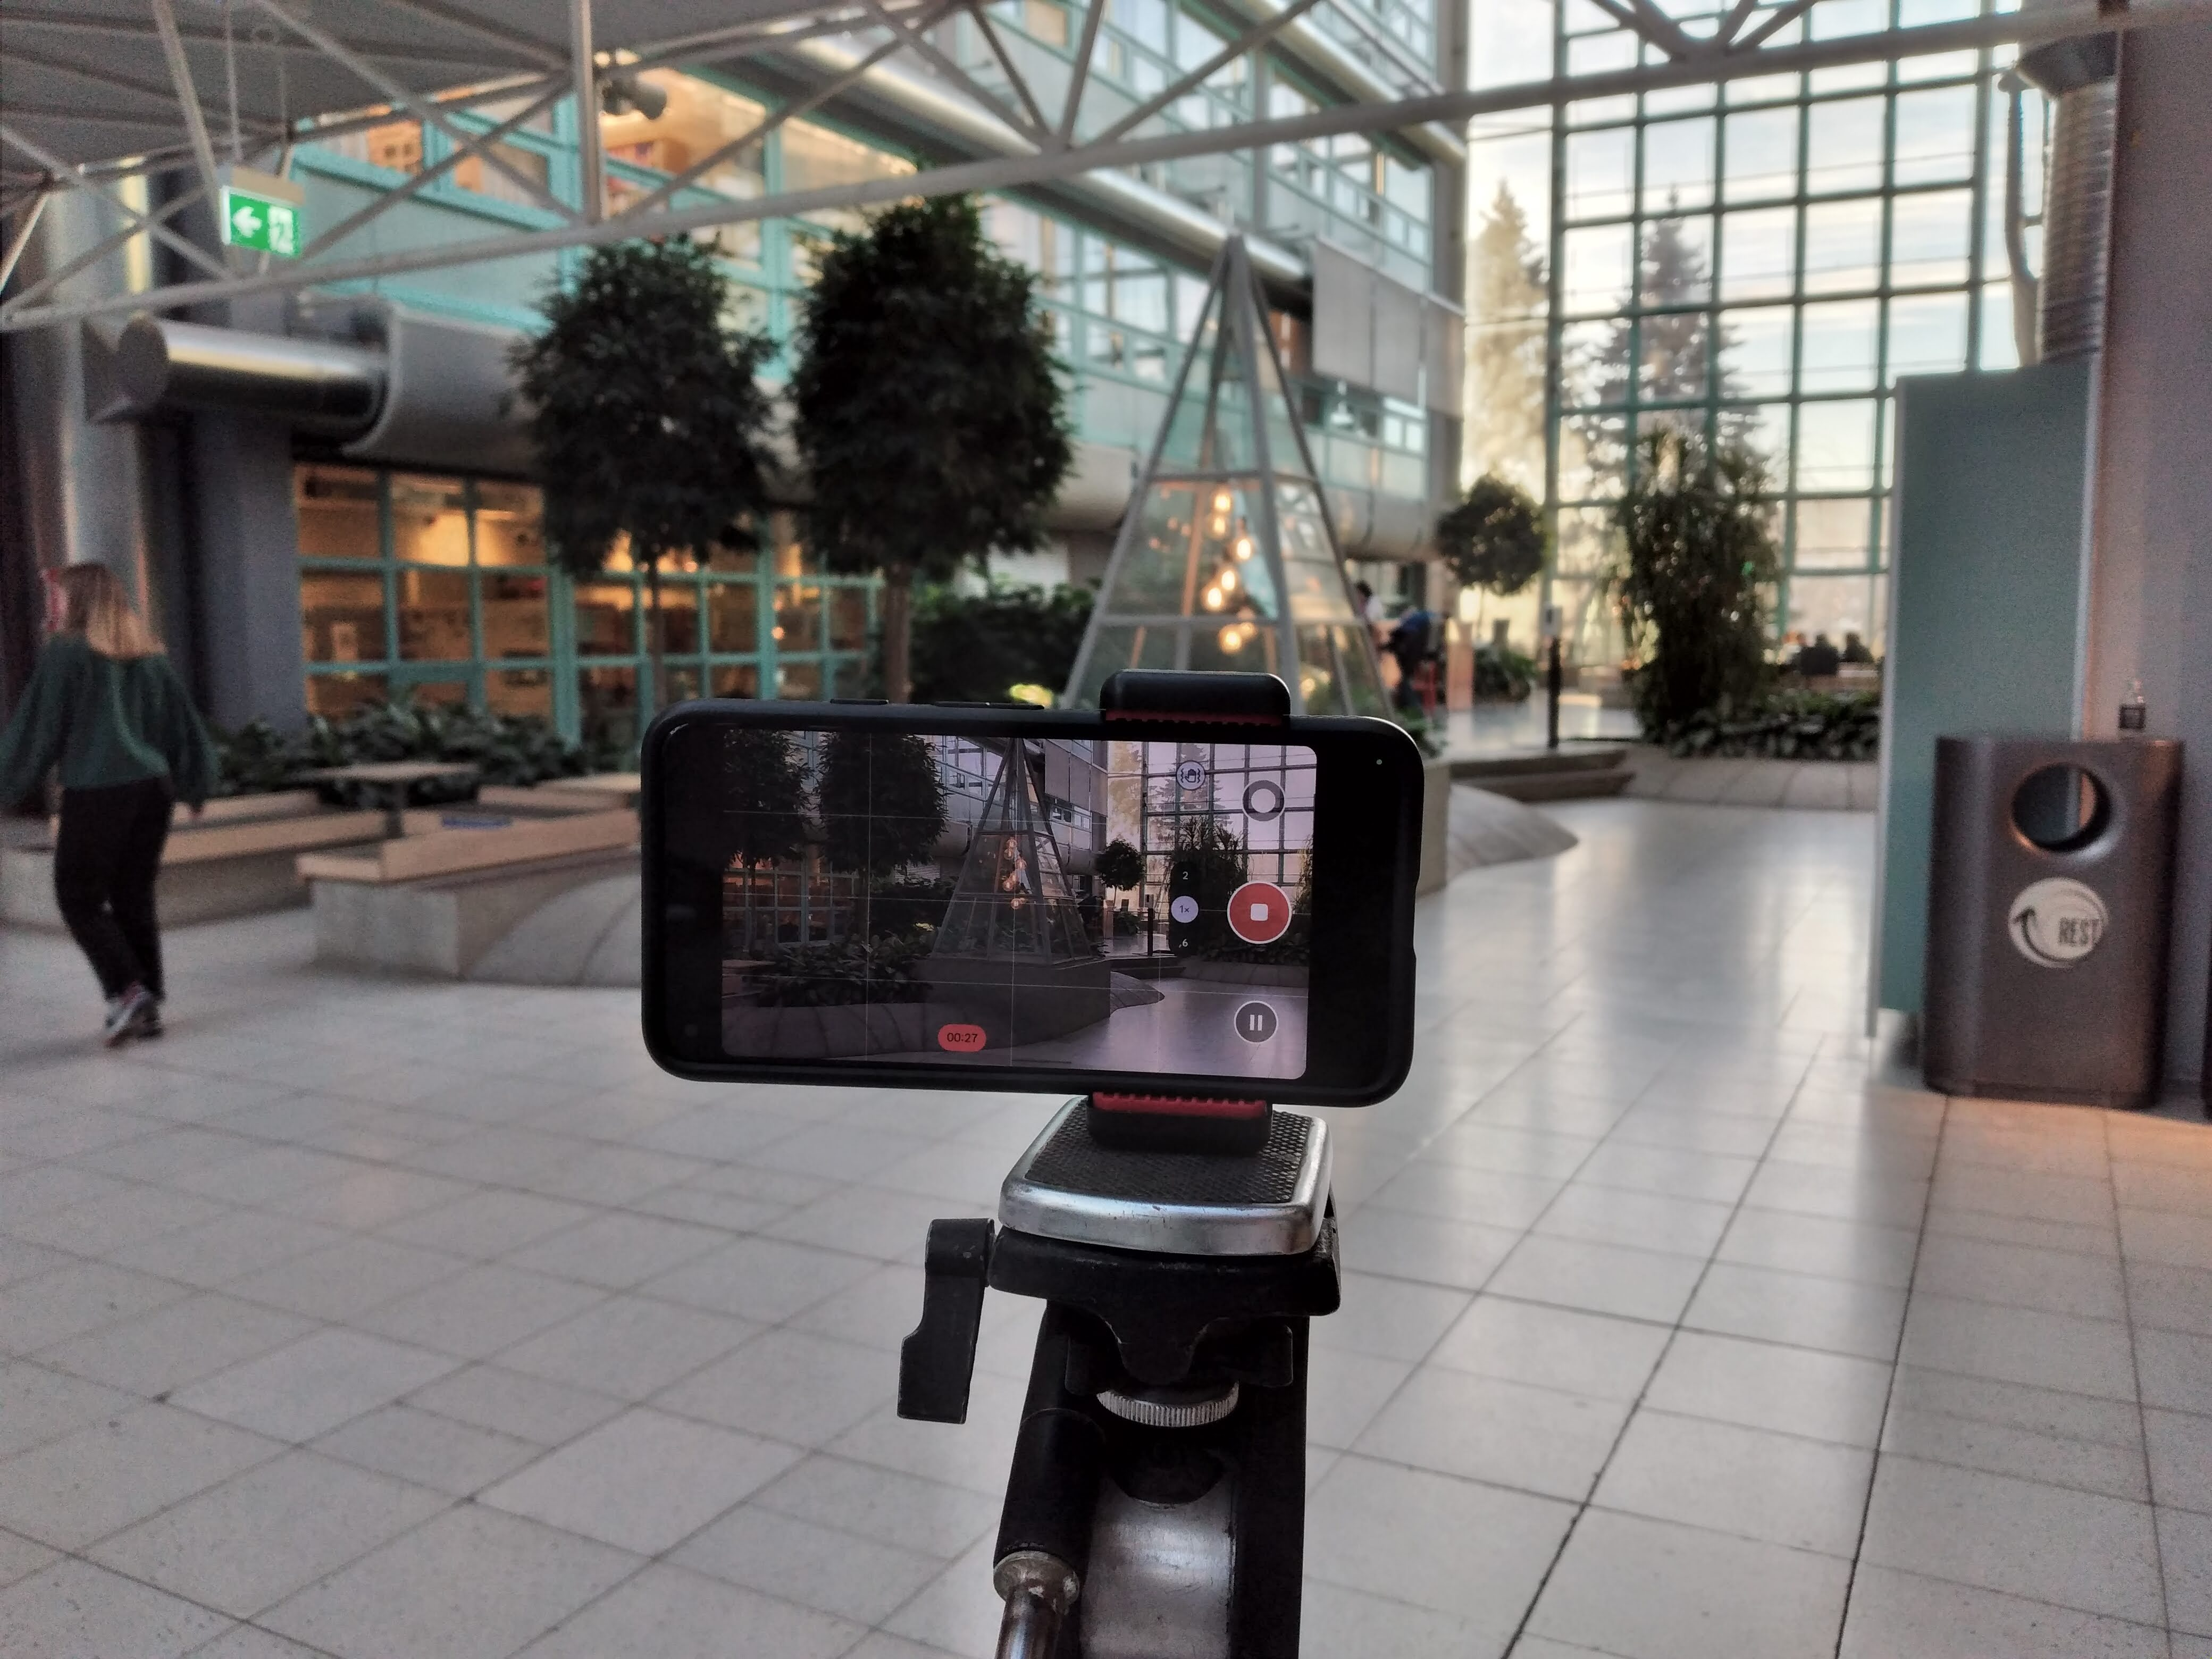
\includegraphics[width=\textwidth]{img/background_setup/windows.jpg}
    \caption{Background  with  windows  to  test for exposure difference and possible movements}
    \label{fig:windows_setup}
\end{figure}


\chapter{Questionnaire}\label{cha:appendix-questionnaire}
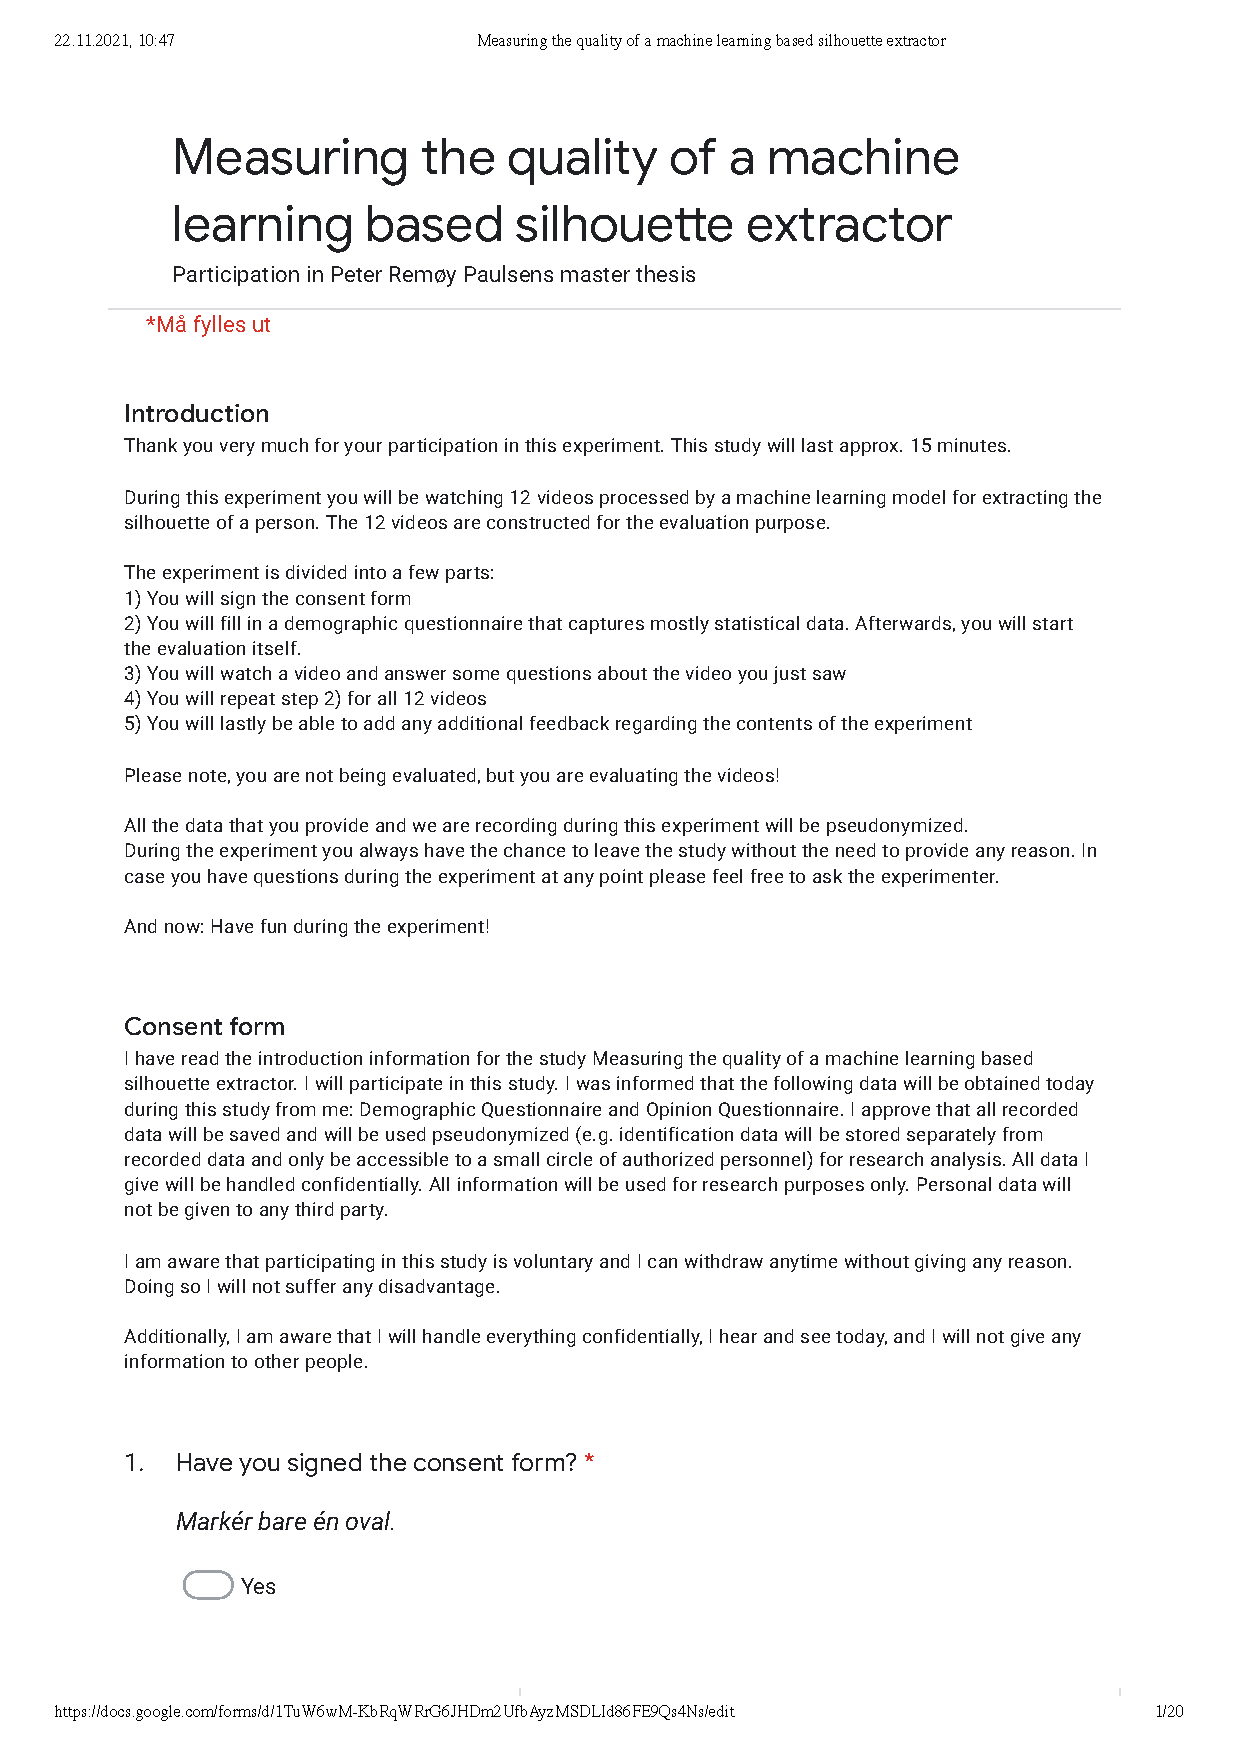
\includepdf[pages=-]{Questionnaires/Questionnaire.pdf}
